% !TeX program = xelatex
% 最终设计中文稿的主文件；沿用现有中文排版框架，目前正文仍有待填写内容。
% 在项目根目录运行 make intermediate，生成 intermediate/preparatory/contract_design_preparation.pdf。
% 本文件字数和页数不限；课程提交版的限制仅在制作提交版时另行核对。
% 面向读者写成品正文；研究推演、核验过程和修改说明不进入可见稿件。
% 未核实的事实、数据、参数、会议与贡献不得写成既定内容。

\documentclass[UTF8,a4paper,11pt,oneside,fontset=fandol]{ctexart}
\usepackage[left=2.25cm,right=2.25cm,top=2.6cm,bottom=2.25cm,headheight=31pt,headsep=16pt,footskip=0.8cm]{geometry}
\usepackage{array,booktabs,tabularx,longtable}
\usepackage{graphicx,caption,placeins,amsmath}
\graphicspath{{research/contract-design/figures/}{../../research/contract-design/figures/}}
\captionsetup[figure]{font=small,labelfont=bf,labelsep=period,position=bottom}
\captionsetup[table]{font=small,labelfont=bf,labelsep=period,position=top}
\renewcommand{\thesection}{\Roman{section}.}
\usepackage{enumitem}
\usepackage{fancyhdr}
\usepackage[backend=biber,style=apa,citestyle=numeric,sorting=nyt]{biblatex}
\addbibresource{research/contract-design/references.bib}
\setlength{\bibitemsep}{\baselineskip}
\usepackage[colorlinks=true,linkcolor=black,urlcolor=black,citecolor=black]{hyperref}
\usepackage{xcolor}
\usepackage{tikz}
\setlength{\parindent}{2em}
\setlength{\parskip}{0.2em}
\setlist[itemize]{leftmargin=2em,nosep}
\renewcommand{\arraystretch}{1.17}
\definecolor{promptgray}{RGB}{100,100,100}
\definecolor{bannerteal}{RGB}{69,131,119} % 参考图主色 #458377
% 参考图的粗黑体视觉；使用 TeX Live 自带黑体保证 make 可移植编译。
\newCJKfontfamily\bannerfont{FandolHei-Bold.otf}
\newcommand{\fillin}[1]{\textcolor{promptgray}{\textbf{【#1】}}}
\newcommand{\sourcehint}[1]{\textcolor{promptgray}{\small #1}}
\newcolumntype{L}[1]{>{\raggedright\arraybackslash}p{#1}}

% 只记录已确认的信息。附件应由真实的三次讨论纪要与实际分工填写后再启用。
\newif\ifIncludeAppendices
\IncludeAppendicesfalse % 完成附件后改为 \IncludeAppendicestrue
\newcommand{\ReportTitle}{广州期货交易所碳期货合约设计}
\newcommand{\RunningTitle}{碳期货合约及规则设计说明}

% 右对齐青绿标题及矢量线框图标，替代原有页眉。
\newcommand{\MarketIcon}{%
  \begin{tikzpicture}[x=0.5pt,y=0.5pt,baseline=-1pt,draw=bannerteal,line width=0.9pt,line cap=round,line join=round]
    \draw (0,0) rectangle (5,11);
    \draw (9,0) rectangle (14,17);
    \draw (18,0) rectangle (23,15);
    \draw (27,0) rectangle (32,24);
    \draw (2,25) -- (11,29) -- (20,26) -- (29,34);
    \foreach \x/\y in {2/25,11/29,20/26,29/34}{\fill[bannerteal] (\x,\y) circle (0.8pt);}
  \end{tikzpicture}%
}
\newcommand{\BannerTitle}{%
  {\color{bannerteal}\bannerfont\fontsize{9}{11}\selectfont\RunningTitle}%
  \hspace{0.6em}\MarketIcon%
}
\pagestyle{fancy}
\fancyhf{}
\fancyhead[R]{\BannerTitle}
\fancyfoot[C]{\thepage}
\renewcommand{\headrulewidth}{0pt}

\begin{document}
\thispagestyle{plain} % 小页眉仅从第二页起显示；第一页保留页码。
\begin{center}
  {\LARGE\bfseries \ReportTitle\par}
\end{center}
\vspace{0.5em}

\section{标的资产与交易品种}
以重点排放单位的配额采购风险作为合约设计的出发点，本合约设计选择全国碳排放配额（CEA）作为广州期货交易所碳期货的标的资产。企业须按照经核查的排放量清缴配额\cite{state2024}；当可用配额低于清缴需求时，企业需要从市场购入差额，未来的配额价格因而直接影响履约成本。CEA 期货为这一采购需求提供提前管理价格风险的工具。2025 年，全国碳市场纳入配额管理的重点排放单位达到 3,378 家，覆盖发电、钢铁、水泥和铝冶炼行业\cite{mee2026}，形成了较为广泛的潜在套期保值需求主体基础。
而对期货标的而言，其还需具备可标准化的资产单位、持续的现货交易基础以及足够的可交割供给，以支持价格形成、期现收敛并降低市场操纵风险。基于这些条件，下文比较 CEA 与 CCER。

\renewcommand{\thesubsection}{\Alph{subsection}.}
\subsection{标准化适配性}
CEA 的标准化优势在于需要处理的资产差异较少，且已有统一发布的市场价格参考。CEA 的资产筛选主要围绕配额年度、登记状态、履约有效性和可划转状态展开\cite{mee2021reg,mee2024carryover}；CCER 除登记与用途约束外，还需处理项目来源、方法学、产生年度及登记批次等差异\cite{ccer2023}。全国注册登记体系使 CEA 的权属与状态能够按统一规则识别\cite{mee2021reg}，合约因而更容易以年度和可用状态界定交割品级。

上海环境能源交易所持续发布 CEA 综合价格行情\cite{she2025daily}，其价格基准的统一性进一步降低了期现价格联系的界定难度；CCER 则存在\textbf{项目间价格差异}，2025 年并网光热和并网海上风电项目的年度成交均价分别为 81.58 和 69.27 元/吨\cite{ccer2025annual}，跨项目均价还会受到成交构成变化的影响。

\subsection{价格波动性}
CEA 价格变化直接影响配额缺口企业的履约采购成本，形成明确的套保需求。2025 年 CEA 综合行情最高价为 97.01 元/吨、最低价为 50.34 元/吨，年末收盘价较上年末下降 23.45\%\cite{she2025annual}；共同交易窗口内，日价格变动标准差为 1.07 元/吨。这表明其采购成本存在可观测、可量化的价格风险。

由图\ref{fig:underlying-liquidity}(a)可见，CCER 价格在较短时期内频繁出现剧烈波动，这将提高每日盯市损益和保证金需求，增加套保企业的资金管理成本；同时，过度波动还可能削弱现货与期货价格关系的稳定性，降低套期保值效果。由图\ref{fig:underlying-liquidity}(b)(c)可见，CCER 的日成交量分布高度集中，前十大成交日占比高达 65.40\%。这意味着 CCER 常态化交易的连续性不足，增加了市场操纵风险。

\subsection{潜在套保需求}
CEA 的潜在买入套保需求来自企业履约前仍需补购的配额。首个履约周期（2019—2020 年度）共有 847 家企业存在配额缺口，占纳管企业的 39.18\%，缺口合计约 1.88 亿吨\cite{mee2022compliance}。近期企业披露进一步体现了采购敞口的规模：长源电力抵扣结存配额后，测算其 2025 年度履约缺口约为 51.12 万吨，并批准于 2026 年采购相应配额\cite{changyuan2026purchase}；按此数量计算，价格每上涨 10 元/吨，采购成本约增加 511.2 万元。因此，缺口企业具有提前锁定 CEA 采购价格的经济需求。

履约采购的价格管理还具有季节性。2024 年第四季度占全年 CEA 成交量的 79\%\cite{mee2025development}；2025 年这一比例达 58.18\%\cite{she2025daily}(图\ref{fig:underlying-liquidity}(d))。年末交易集中驱使企业在履约前提前管理采购价格风险。

\begin{table}[!htbp]
\centering
\small
\setlength{\tabcolsep}{5pt}
\renewcommand{\arraystretch}{1.10}
\caption{CEA 与 CCER 的交易基础、活跃程度与流动性指标}\label{tab:underlying-liquidity}
\begin{tabular}{@{}L{0.34\textwidth}L{0.30\textwidth}L{0.30\textwidth}@{}}
\toprule
指标 & CEA & CCER\\
\midrule
\multicolumn{3}{@{}l}{\textit{A. 交易基础与参与者}}\\
供给及需求基础 & 年度配额分配；强制清缴\cite{state2024} & 项目核证登记；合规抵销5\%\cite{ccer2023}\\
实际参与交易主体 & 1,471 家（2024 年）\cite{mee2025development} & 90 家（截至2025年8月累计）\cite{mee2025development}\\
\addlinespace
\multicolumn{3}{@{}l}{\textit{B. 共同窗口挂牌成交}}\\
成交量（万吨） & 7,901.17 & 884.41\\
成交额（亿元） & 49.49 & 6.26\\
日成交量中位数（吨） & 288,406 & 2,700\\
日成交量 $\leq$1,000 吨（天） & 5 & 72\\
前十大成交日占比（\%） & 16.35 & 65.40\\
第四季度成交量占比（\%） & 58.93 & 68.28\\
\addlinespace
\multicolumn{3}{@{}l}{\textit{C. 标准化流动性指标}}\\
Amihud \textsuperscript{a} & 0.001197 & 13.059870\\
日价格变动标准差（元/吨）\textsuperscript{b} & 1.07 & 7.14\\
\bottomrule
\multicolumn{3}{@{}p{0.97\textwidth}@{}}{\footnotesize
\textit{注：}采用 2025 年 3 月 7 日至 12 月 31 日的 203 个共同交易日及挂牌口径，日量指标保留零成交日。
\textsuperscript{a}Amihud 为 $|r_t|/(A_t/10^6)$ 的样本均值\cite{amihud2002}，$r_t$ 为小数形式简单收益率，$A_t$ 为当日成交额（元）；只保留相邻交易日且两日有挂牌成交的价格对。CEA 使用综合收盘价，CCER 使用跨项目日均价；二者价格定义不同，此处仅用于论证 CEA 更适合期货标的。
\textsuperscript{b}日价格变动为相邻交易日价格之差，仅保留两日均有挂牌成交的价格对。
\textit{来源：}CEA 交易及价格数据\cite{she2025daily}；CCER 总量及成交额\cite{ccer2025annual,ccer2025dec30,ccer2024jan22}；CCER 日度交易及价格数据\cite{ccn2025daily}，按官方公告更正\cite{ccer2025jun24,ccer2025jul01}。B、C 组统计指标由本文计算。}\\
\end{tabular}
\end{table}
\FloatBarrier

\begin{figure}[!htbp]
  \centering
  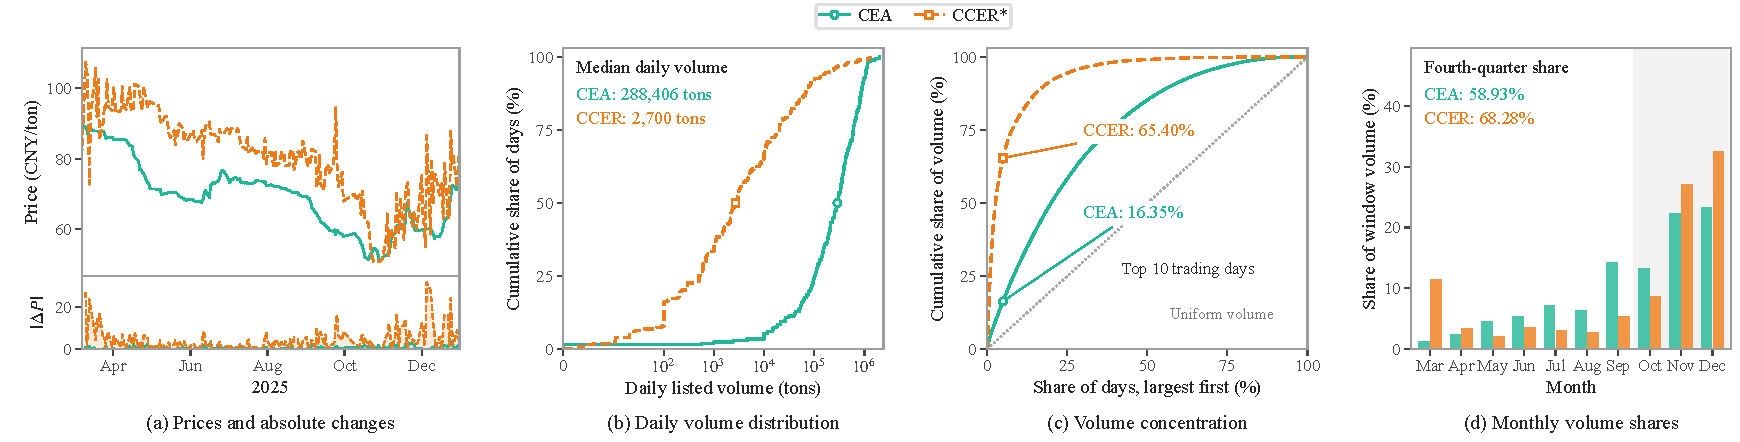
\includegraphics[width=\textwidth]{step2_liquidity_four_panel.pdf}
  \caption{CEA 与 CCER 的价格变化及挂牌成交分布}
  \label{fig:underlying-liquidity}
  \begin{minipage}{\textwidth}
    \footnotesize
    \textit{注：}样本为 2025 年 3 月 7 日至 12 月 31 日的 203 个共同交易日，保留零成交日；CCER 二次日表较官方累计量少 9,020 吨，日度分布按现有整理样本计算。(a) 上栏为 CEA 综合收盘价与 CCER 日成交均价，下栏为各自相邻观测日的绝对价差 $|P_t-P_{t-1}|$，单位均为元/吨。(b) 日成交量经验累积分布，横轴采用对数坐标，刻度为吨；(c) 将交易日按日量从高到低排序后计算累计成交占比，标记前十日，灰色对角线表示各日等量；(d) 月成交量占各市场样本总量的比例，灰色背景标识第四季度。\textit{来源：}上海环境能源交易所逐日公告\cite{she2025daily}；碳中和网逐日整理表\cite{ccn2025daily}，按全国 CCER 交易系统公告更正\cite{ccer2025jun24,ccer2025jul01}。本文计算。
  \end{minipage}
\end{figure}
\FloatBarrier

\subsection{标的与可交割配额范围}
本合约以最近履约年度 CEA 为基准交割品，即交割当年须完成清缴的排放年度配额，具体年度在合约挂牌时锁定。例如，2026 年履约对应 2025 年度排放，基准品为 2025 年度 CEA\cite{mee2026work}。替代品限于生态环境部规定对该履约年度具有同等清缴效力、且已完成必要结转登记的其他年度 CEA；现行规则允许 2026 年度配额用于 2025 年度清缴\cite{mee2026allocation}。2019—2024 年度配额须按规定回收并换发为 2025 年度配额后方可纳入，未结转旧额不合格\cite{mee2024carryover,mee2026allocation}。

交割配额须登记在卖方本人名下、正常可用的全国碳排放权登记账户中；买卖双方均须具备现货持有、转让或受让资格及交易所交割资格\cite{mee2021reg}。本方案排除已清缴、注销、冻结、质押及其他限制划转的配额，也排除处于清缴、注销或结转申请锁定状态的配额；相关限制解除后须重新核验。基准品与合格替代品可按吨等量混合交割，但须逐年度申报并分别核验，保证全部配额对同一履约年度有效。若政策改变履约效力或结转条件，交易所应按新规更新合格清单，失效品须更换；若无有效替代品，则依预先公布的应急规则暂停受影响交割并处置存量合约。

\clearpage
\section{标准化合约条款}
% 每一行：设计内容给出可执行值/规则；设计依据给出逻辑、数据或制度来源。
% 原件表头：Term | Design Content | Design Basis。提交前删除全部提示词。
\small
\begin{longtable}{@{}L{0.225\textwidth}L{0.265\textwidth}L{0.445\textwidth}@{}}
\caption{拟议碳期货合约条款表}\label{tab:contract}\\
\toprule
\textbf{条款（Term）} & \textbf{设计内容（Design Content）} & \textbf{设计依据（Design Basis）}\\
\midrule
\endfirsthead
\toprule
\textbf{条款（Term）} & \textbf{设计内容（Design Content）} & \textbf{设计依据（Design Basis）}\\
\midrule
\endhead
\bottomrule
\endfoot
交易品种及代码 & 全国碳排放配额期货；拟议代码 CE & 名称限定全国 CEA，与地方试点配额及 CCER 区分。CE 取 Carbon Emission 首字母，参照现有合约采用两字母形式\cite{gfexProductCodes2026}，与 SI、LC、PS、PT、PD 区分；正式代码由交易所确定。\\
交易单位 & 1,000 吨二氧化碳当量/手 & 参照 EUA 期货规格及国内 10 万吨实际采购案例\cite{iceEuaSpecs,sinopec2021bulk}；该规模对应 100 手，最近整数取整偏差至多 500 吨。按 2025 年末 74.63 元/吨\cite{mee2026}估值为 74,630 元/手。\\
报价单位 & 人民币元/吨二氧化碳当量 & 与 CEA 的统一计量\cite{state2024}及现货价格口径\cite{she2025daily}一致；一手盈亏等于价格变动乘以 1,000 吨。\\
最小变动价位 & 0.01 元/吨二氧化碳当量 & 与全国 CEA 现货申报价格精度一致\cite{mee2021trade}；按 1,000 吨/手计算，每跳盈亏为 10 元，保留分位报价和细小价格调整空间。\\
每日价格涨跌停板 & 上一交易日结算价的 $\pm6\%$；10—12 月为 $\pm10\%$。单边市后扩板及恢复规则见下文。 & 据 2025 年现货日数据\cite{she2025daily}计算，219 组有效相邻日绝对变动的第 99 百分位为 5.36\%，支持常态 6\%；第四季度最大为 8.26\%，据此将履约窗口放宽至 10\%；扩板参照广期所风险管理办法\cite{gfexRisk2022reprint}。\\
最低交易保证金 & 合约价值的 8\%；10—12 月为 12\%；最后交易日前第 5 个交易日起为 20\%。异常扩板时按第 IV 节取高。 & 8\%、12\% 分别高于 6\%、10\% 停板幅度 2 个百分点；现货两日累计绝对变动最大值在前三季度、第四季度分别为 5.46\%、9.91\%\cite{she2025daily}（本文计算）。临近到期另留流动性缓冲，配合逐日盯市与追缴。\\
合约月份 & \fillin{月份及挂牌跨度} & \fillin{套保周期、分配/清缴日历与流动性依据}\\
最后交易日 & \fillin{可执行的交易日定义} & \fillin{价格发布或资产划转所需时间及节假日处理}\\
交割方式 & 实物交割；每手交付 1,000 吨合格 CEA，通过全国注册登记系统完成权属转移。 & 全国登记制度已有电子确权与现货货银对付基础；在第 III.A 节 A1—A3 下衔接期货交割，直接满足履约资产采购。\\
交割品级/标准 & \fillin{合格资产或现金指数样本范围} & \fillin{年度/批次、登记状态、排除条件与价格源一致性}\\
\end{longtable}
\normalsize

本方案的合约标识由拟议品种代码 CE 与四位到期年月 YYMM 组成；年月后缀表示合约到期月份，可交割配额的排放年度则按第 I.D 节在挂牌时另行锁定。

交易单位设为每手 1,000 吨二氧化碳当量。国际上，ICE Endex 的 EUA 期货每手为 1,000 份配额，每份对应 1 吨二氧化碳当量\cite{iceEuaSpecs}；国内已有十万吨级实际采购，例如中国石化于 2021 年 7 月 21 日从华润集团购入 10 万吨 CEA\cite{sinopec2021bulk}，按本方案可对应 100 手。整数手数匹配下的最大数量偏差为 500 吨，即对 10 万吨敞口仅为 0.5\%。该规模在套保粒度与单份合约金额之间取得平衡，具体条款见第 II 节。


最小变动价位设为 0.01 元/吨二氧化碳当量，与全国 CEA 现货申报价格的最小变动计量一致\cite{mee2021trade}。按每手 1,000 吨计算，0.01、0.05 和 0.10 元/吨分别对应每跳 10、50 和 100 元；采用 0.01 元可保留现货分位报价，便于细化套保成交价格。ICE EUA 期货同为每手 1,000 吨，最小价位为 0.01 欧元/吨、每跳 10 欧元\cite{iceEuaSpecs}，可作规格结构参照；人民币与欧元的每跳金额不作等值比较。实际成交成本仍取决于买卖价差、盘口深度及交易费用，后续应据实际交易数据评估价位是否需要调整。


每日涨跌停板的常态幅度设为上一交易日结算价的 $\pm6\%$。按相邻两个交易日均有挂牌成交的口径，2025 年全国 CEA 综合收盘价构成 219 组有效日变动，绝对变动第 99 百分位为 5.36\%；4\%、5\% 和 6\% 的候选幅度分别被超过 6、5 和 1 次\cite{she2025daily}（本文计算）。6\% 为常态价格调整保留空间。第四季度的 60 组观测中，最大变动达 8.26\%，高于前九个月的 5.29\%；2025 年配额清缴截止日为 12 月 31 日\cite{mee2025work}。本方案因此按交易日期将 10—12 月所有挂牌合约的常态幅度提高至 $\pm10\%$，为履约前较大的价格调整留出余量；若清缴日历改变，则提前公告调整适用窗口。这些现货收盘价统计用于选择初始幅度，尚不能代表指定年度期货的日内波动或实际触板频率。

设上一交易日的期货结算价为 $P$、当日适用幅度为 $L$，涨停价按 $P(1+L)$ 向下取至 0.01 元，跌停价按 $P(1-L)$ 向上取至 0.01 元，使报价格点不超出规定幅度；挂牌首日以交易所公布的挂牌基准价代替 $P$。例如，$P=74.63$ 元时，6\% 幅度对应 70.16—79.10 元，10\% 对应 67.17—82.09 元。每日结算价的计算方法另见第 III 节，现货收盘价仅用于本节历史分析。

异常调整参照广期所风险管理办法的单边市机制\cite{gfexRisk2022reprint}：收盘前五分钟持续封在停板、只有停板方向申报而无有效对手报价时，认定为单边市，盘中短暂触板不触发扩板。首个单边市日记为 D1，D2 幅度在 D1 实际幅度上加 3 个百分点；D2 再现同向单边市，D3 再加 2 个百分点。由此，6\% 起点对应 9\%、11\%，10\% 起点对应 13\%、15\%。未再出现单边市时，下一交易日恢复当期常态幅度；反向单边市作为新一轮 D1，在当日实际幅度上重新调整。季节、单边市与专项公告同时适用时取较高幅度。扩板须在下一交易日开市前完成保证金调整与追缴，异常保证金不低于适用幅度加 2 个百分点及本轮 D1 前结算时的比例，基础与临近到期保证金比例见第 IV 节。连续三个同向单边市后，交易所应公告限制开仓、继续调幅或暂停交易等处置；临近到期时维持已公告的到期安排，不能依靠延期自动消除风险。

放宽停板只能增加可报价范围，无法保证成交或平仓。假设每日均在停板价结算，6\%、9\%、11\% 三日连续上涨的累计涨幅为 28.25\%；10\%、13\%、15\% 路径则为 42.95\%（本文情景计算，未计报价取整）。因此，保证金及可用资金安排须承受连续扩板后的累积损失，不能把单日停板幅度当作最大损失。


\section{交割机制与参考、结算价格}
\subsection{交割方式的选择}
本合约兼顾履约采购价格管理与到期取得合格 CEA，交割方式须满足登记结算与可交割供给的要求。

实物交割通过登记账户划转配额，可直接完成约定数量的履约资产采购，但需要跨系统交收，并承担卖方违约、系统故障和库存集中风险。现金交割仅结清价差，免除期货项下的配额划转，降低跨系统操作依赖；在结算基准可靠且具有代表性时，可以管理价格风险，但企业仍须另行采购配额，并承担采购价格偏离基准的基差风险和配额不足的风险。

全国 CEA 已具备电子交付的制度基础：配额归属以注册登记系统记录为准，登记机构可核验持有数量和状态，并按成交结果办理变更\cite{mee2021reg}；现货结算按货银对付原则完成清算、交收和对账\cite{mee2021settlement}。现货基础仍需与期货配对指令、资金结算和配额锁定机制衔接。方案成立仍需满足以下假设：
\begin{enumerate}
\item \textbf{A1：交割接入。}合约取得必要批准，交割双方具备相应资格；经授权的衔接机制能够接收期货配对结果，核验并锁定配额，防止重复处分，完成划转并出具回执。
\item \textbf{A2：资金与系统协调。}货款备付、配额划转和对账遵循货银对付原则，期货盯市盈亏与交收货款分别核算；指令失败、重复提交和系统中断有补正安排，买方可在清缴截止前取得可用配额。
\item \textbf{A3：供给与持仓匹配。}能够核验合格配额的可用余额及持有集中度，并据此约束到期持仓；交付时配额具有清缴效力、已完成必要结转且无划转限制。
\end{enumerate}

在 A1—A3 下，本合约选择\textbf{实物交割}，直接衔接履约资产采购：卖方每手交付 1,000 吨符合第 I.D 节的 CEA，买方支付交收货款，以登记系统完成权属变更并出具回执确认交付。若上述条件无法落实，应在挂牌前重新评估方案；现金交割也须独立满足结算基准的使用与质量要求，不能在实物交割失败后自动启用。

\noindent\textbf{每日结算价：}\fillin{期货成交数据来源、计算窗口和公式、发布时间、无成交/异常时规则}。

\noindent\textbf{到期最终价格：}\fillin{交割结算价或现金最终结算价的数据来源、公式、观察窗口、发布时间、修正/备用规则}。
说明该价格如何与标的现货收敛；不要将现货收盘价、期货每日结算价和到期价格混用。

\section{风险管理}
\noindent\textbf{保证金与逐日盯市：}基础交易保证金设为合约价值的 8\%，10—12 月提高至 12\%，分别在当期 6\%、10\% 停板幅度上保留 2 个百分点。按连续三个交易日均有挂牌成交的口径，2025 年现货两日累计绝对价格变动的最大值，前三季度为 5.46\%、第四季度为 9.91\%\cite{she2025daily}（本文计算）；8\%、12\% 为这两种历史情景留出余量。两日是初步压力观察窗口，不能据此认定实际持仓可在两日内平仓；保证金仍需兼顾流动性、季节性和前瞻事件风险\cite{cmeMarginModel}。从最后交易日前第 5 个交易日起提高至 20\%，直至相应结算交收完成。该操作窗口用于提前核验资金与交收准备；20\% 在样本三日最大变动 14.26\% 上另留缓冲，其比例与时点须结合最终交割流程复核。

单边市期间，保证金取当期基础或季节比例、临近到期比例、下一交易日停板幅度加 2 个百分点、本轮 D1 前结算时比例及专项公告标准中的最高值\cite{gfexRisk2022reprint}。不涉及临近到期或其他提高条件时，常态连续扩板对应保证金 8\%、11\%、13\%，第四季度对应 12\%、15\%、17\%；进入临近到期窗口后仍至少为 20\%。反向单边市重新起算，连续三个同向单边市后在专项处置公告前不自动下调；无单边市后可恢复当期常态标准，但仍须保留其他有效的较高标准。节假日、政策变化或流动性明显恶化时，应提前公告提高保证金，必要时在盘中追缴；这些提高条件对套保持仓同样适用。

每手保证金金额等于 1,000 吨乘以计价结算价及适用比例。以 74.63 元/吨的历史价格示例，8\%、12\% 和 20\% 分别为 5,970.40、8,955.60 和 14,926.00 元/手。方案采用逐日盯市：每日亏损与新增保证金占用分别计入资金需求；预定提高在生效日前一交易日结算时，对存量持仓按当日结算价收取新比例，下一交易日开市前补足，进入较高标准窗口后新挂牌的合约从首日起适用该标准。期货公司向客户收取的比例不得低于交易所标准，并应安排更早的客户追缴时限\cite{gfexSettlement2025reprint}。未补足时限制开仓，并按规则处置持仓；停板无法平仓时仍须追索欠款与启动违约处置，不假定强行平仓必然成交。结算交收资金另按第 III 节的最终方案准备，交易保证金不能代替应付交收款。

连续扩板还会同时增加盯市损失与保证金占用。假设一手空头以 74.63 元起始、账户只存最低保证金，每日均按涨停价结算并及时补款，三日 6\%、9\%、11\% 路径产生 21,082.53 元累计亏损；除初始 5,970.40 元外，合计还须补入约 27,554.76 元，期末保留 13\% 的交易保证金。第四季度 10\%、13\%、15\% 路径则在初始 8,955.60 元外追加约 41,229.83 元，期末保留 17\%（本文情景计算，第三日后暂维持原比例，未计报价取整、费用及更高专项要求）。因此，8\% 与 12\% 是进入持仓的保证金下限，持续持仓还依赖可及时调入的资金；不具备补款能力的主体应提前减仓。

\noindent\textbf{涨跌停板：}执行第 II 节的季节性幅度、单边市扩板及恢复规则，并与保证金追缴联动。

\noindent\textbf{持仓限额：}\fillin{一般月份、临近到期月份的额度、主体合并及套保处理}。

\noindent\textbf{大户报告：}\fillin{触发阈值、报告内容、时点和核查程序}。

\noindent\textbf{履约周期：}\fillin{所选标的适用的清缴/注销时间、潜在价格和供应冲击；保证金及限仓调整触发条件}。
简述登记/价格源停机、无成交、政策改变合格资产、持仓集中时的备用措施，并与表\ref{tab:contract}及交割条款一致。

\section*{参考文献}
\printbibliography[heading=none]

% 附件仅在有真实讨论记录与成员贡献资料后加入。
\ifIncludeAppendices
\clearpage
\appendix
\section{小组讨论纪要}
% 必须是三次真实的正式讨论；复制下方段落并据真实记录填写。
\subsection*{第一次讨论}
\noindent 时间/地点/参加人：\fillin{据真实记录填写}。\par
\noindent 议题与依据：\fillin{据真实记录填写}。\par
\noindent 主要意见、决策过程与待办：\fillin{据真实记录填写}。\par
\subsection*{第二次讨论}
\noindent 时间/地点/参加人：\fillin{据真实记录填写}。\par
\noindent 议题与依据：\fillin{据真实记录填写}。\par
\noindent 主要意见、决策过程与待办：\fillin{据真实记录填写}。\par
\subsection*{第三次讨论}
\noindent 时间/地点/参加人：\fillin{据真实记录填写}。\par
\noindent 议题与依据：\fillin{据真实记录填写}。\par
\noindent 主要意见、决策过程与待办：\fillin{据真实记录填写}。\par

\section{成员分工说明}
% 每人至少独立撰写一个核心模块；只填实际工作与可核实贡献。
\noindent\fillin{逐名列出独立撰写的核心模块、研究/数据/整合工作及实际贡献}。
\fi
\end{document}
